
% This LaTeX was auto-generated from MATLAB code.
% To make changes, update the MATLAB code and republish this document.

\documentclass{article}
\usepackage{graphicx}
\usepackage{color}

\sloppy
\definecolor{lightgray}{gray}{0.5}
\setlength{\parindent}{0pt}

\begin{document}

    
    \begin{verbatim}
errors = zeros(numSims,1);
for k=1:numSims
    errors(k) = Experiment_Output{k,6};
end

figure
plot(errors)
title('Error vs iteration number')

display(['The standard deviation of error is ',num2str(std(errors))])
display(['The min and max error are respectively ', num2str(min(errors)), ' ', num2str(max(errors)) ])

% , ' ' , num2str(max(errors))
\end{verbatim}

        \color{lightgray} \begin{verbatim}The standard deviation of error is 0.00053162
The min and max error are respectively 5.8434 5.8512
\end{verbatim} \color{black}
    
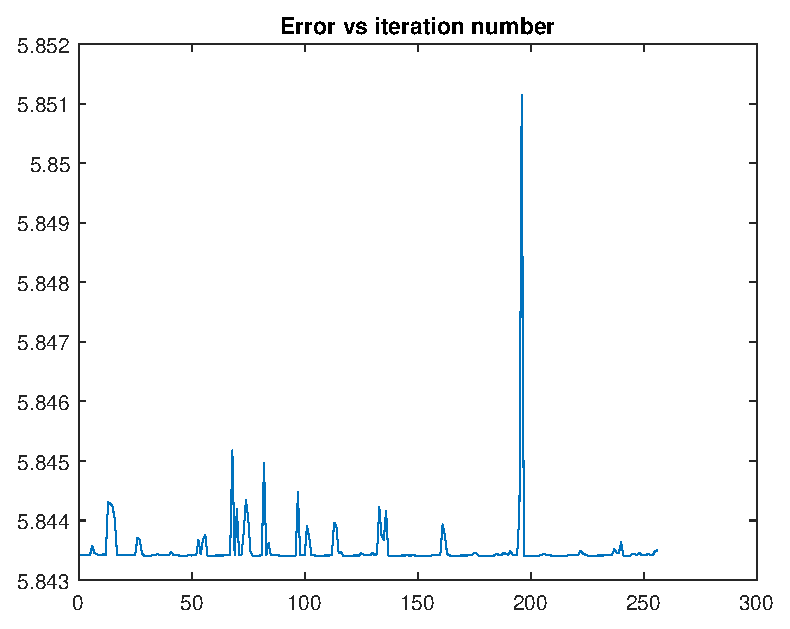
\includegraphics [width=4in]{error_spread_01.eps}
\begin{verbatim}
[error_min,min_index] = min(errors);
[error_max,max_index] = max(errors);

% - 3rd column is output of fmincon, {exitflag, output, lambda, grad, hessian};"

fminconOutput_min =  Experiment_Output{min_index, 3};
exitflag_min = fminconOutput_min{1};

gradient_min = fminconOutput_min{4};
hessian_min = fminconOutput_min{5};

%
fminconOutput_max =  Experiment_Output{max_index, 3};
exitflag_max = fminconOutput_max{1};
f_max
gradient_max = fminconOutput_max{4};
hessian_max = fminconOutput_max{5};
\end{verbatim}

        \color{lightgray} \begin{verbatim}Unrecognized function or variable 'f_max'.

Error in error_spread (line 31)
f_max 
\end{verbatim} \color{black}
    \begin{verbatim}
display( fminconOutput_min{2});
display( fminconOutput_max{2});
\end{verbatim}



\end{document}

